\documentclass[12pt]{article}
\usepackage{geometry}
 \geometry{
 a4paper,
 total={170mm,257mm},
 left=20mm,
 top=20mm,
 }

 \setlength{\headheight}{30.0pt}
\setlength{\footskip}{20pt}

 \usepackage[export]{adjustbox}
\usepackage[english]{babel}
\usepackage[utf8]{inputenc}
\usepackage{fancyhdr}
\usepackage{multicol}
\pagestyle{fancy}
\fancyhf{}
\rhead{\textit{LAB -3}}
\lhead{\textit{Pul074BEX004}}
\rfoot{\thepage}


\usepackage{mathpazo} % Palatino font
\usepackage{graphicx}
\usepackage{float}

%%%% Anser environment use %%%% Anser environment use %%%% Anser environment use \input{./AnsENV.tex}
%% use \begin{A... {**** argument***}
\RequirePackage{scrextend}

\newenvironment{A}[1]{\textit{Answer:}{\begin{addmargin}[2em]{2em}{#1}\end{addmargin} 
  }}

% just leave some space   
%% use \begin{A... {**** argument***}
\RequirePackage{scrextend}

\newenvironment{A}[1]{\textit{Answer:}{\begin{addmargin}[2em]{2em}{#1}\end{addmargin} 
  }}

% just leave some space   
%% use \begin{A... {**** argument***}
\RequirePackage{scrextend}

\newenvironment{A}[1]{\textit{Answer:}{\begin{addmargin}[2em]{2em}{#1}\end{addmargin} 
  }}

% just leave some space    %% Answer environment 

%%% Question Environment%%%  use 
%%% Question Environment%%%  use 
%%% Question Environment%%%  use \input{./QueENV.tex}   to include
%% Use \begin{Q}....\end{Q}

\newcounter{QC}
\setcounter{QC}{1}
\newenvironment{Q}[1]{
    \section{Question -\arabic{QC}} \stepcounter{QC}{\large\textbf{#1}}
}

%%% Question Environment%%%

   to include
%% Use \begin{Q}....\end{Q}

\newcounter{QC}
\setcounter{QC}{1}
\newenvironment{Q}[1]{
    \section{Question -\arabic{QC}} \stepcounter{QC}{\large\textbf{#1}}
}

%%% Question Environment%%%

   to include
%% Use \begin{Q}....\end{Q}

\newcounter{QC}
\setcounter{QC}{1}
\newenvironment{Q}[1]{
    \section{Question -\arabic{QC}} \stepcounter{QC}{\large\textbf{#1}}
}

%%% Question Environment%%%

 %% Question Environment 
%%%%%% include  Titles.%%%% use \input{./CP}%%%
%%%use """"""""    \CP{}{}{}{}   """" %%%% and 4 argument to craete Title page 
%%%%%%%%%%%%%%%%%%%%%%%%%%%%%%%%%%%%%%%%%%%%%%%%%%%%%%%%%%%%%%%%%
%%%argument number
%% 1=major header ## Course name 
%% 2=minor4 heading ## lab/assignmet no
%% 3=Title  ## Assignment or Lab title
%% 4=submitted to::## input receiver Name"
%%%%%%%%%%%%%%%%%%%%%%%%%%%%%%%%%%%%%%%%%%%%%%%%%%%%%%%%%%%%%%%%%


\usepackage{mathpazo} % Palatino font
\usepackage{graphicx}
\usepackage{float}

%%% format and command for lab ans c and assembly

\newcommand{\HRule}{\rule{\linewidth}{0.4mm}} % Defines a new command for horizontal lines, change thickness here



%----------------------------------------------------------------------------------------
%	TITLE PAGE
%----------------------------------------------------------------------------------------


\newcommand{\CP}[4]{ \begin{titlepage} % Suppresses displaying the page number on the title page and the subsequent page counts as page 1
		%%%%  univerdity logo%%
		\begin{figure}[H]
			\centering
			
\includegraphics[scale=0.13]{tulogo.jpg}
		\end{figure}
		%%% end university logo

		\center % Centre everything on the page

		%------------------------------------------------
		%	Headings
		%------------------------------------------------

		\textsc{\huge Institute of Engineering \\ Central Campus,Pulchowk}\\[1.5cm] % Main heading such as the name of your university/college

		\textsc{\Large #1}\\[0.5cm] % Major heading such as course name

		\textsc{\large #2}\\[0.5cm] % Minor heading such as assignment no./ lab no.

		%------------------------------------------------
		%	Title
		%------------------------------------------------

		\HRule\\[0.4cm]

		{\Huge\bfseries #3}\\[0.4cm] % Title of your document

		\HRule\\[1.5cm]

		%------------------------------------------------
		%	Author(s)
		%------------------------------------------------
		\vfill\vfill
		\begin{minipage}{0.4\textwidth}
			\begin{flushleft}
				\large{
				\textbf{Submitted BY:}\\
				{\normalsize AMRIT PRASAD PHUYAL}\\ % NAME
				{\normalsize Roll: PULL074BEX004}} % Roll
			\end{flushleft}
		\end{minipage}
		~
		\begin{minipage}{0.4\textwidth}
			\begin{flushright}
				\large
				\textbf{Submitted To:}\\
				{ \normalsize{#4}\\ }% recepent's  Name 
				{\normalsize Department of Electronics and Computer Engineering}
			\end{flushright}
		\end{minipage}

		%------------------------------------------------
		%	Date
		%------------------------------------------------

		\vfill\vfill\vfill % Position the date 3/4 down the remaining page

		{\large\today} % Date, change the \today to a set date if you want to be precise

		\vfill % Push the date up 1/4 of the remaining page

	\end{titlepage}
} %%% cover page

%%% For CMD output %%%

%%%%%%%%% use  
%%% For CMD output %%%

%%%%%%%%% use  
%%% For CMD output %%%

%%%%%%%%% use  \include{CMD output.tex}
%%%%%%%%% use \CMD{###filename}{##Caption}
\usepackage{listings}

\usepackage{mdframed}
\usepackage{xcolor}
%\definecolor{codegreen}{rgb}{0,0.6,0}
%\definecolor{codegray}{rgb}{0.4,0.4,0.4}
%\definecolor{codepurple}{rgb}{0.58,0,0.82}
%\definecolor{blackcolour}{rgb}{0,0,0}


\definecolor{bluefront}{RGB}{10,214,255}
\definecolor{blueback}{RGB}{25,24,96}


\renewcommand{\lstlistlistingname}{List of CMD Outputs}
\renewcommand{\lstlistingname}{Output}


\lstdefinestyle{customa}{
    backgroundcolor=\color{blueback},
    %  keywordstyle=\color{magenta},
    %numberstyle=\tiny\color{codegray},
    %stringstyle=\color{codepurple},
    basicstyle=\ttfamily\scriptsize\color{bluefront},
    breakatwhitespace=false,
    breaklines=true,
    captionpos=b,
    %morekeywords={MOV,ADD,ADDC,ACALL,INC,DJNZ,AJMP,RET,END,ORG,RR,JNC,SUBB,JC,DEC},
    keepspaces=true,
    %numbers=left,
    %numbersep=5pt,
    showspaces=false,
    showstringspaces=false,
    showtabs=false,
    tabsize=4
}

\newcommand {\CMD}[2]{

    \begin{mdframed}[backgroundcolor=blueback,innerbottommargin=-2.3em,innertopmargin=-0.1em]
        \lstinputlisting[style=customa,caption={#2}]{#1}
    \end{mdframed}
}

%%% For CMD output %%%


%%%%%%%%% use \CMD{###filename}{##Caption}
\usepackage{listings}

\usepackage{mdframed}
\usepackage{xcolor}
%\definecolor{codegreen}{rgb}{0,0.6,0}
%\definecolor{codegray}{rgb}{0.4,0.4,0.4}
%\definecolor{codepurple}{rgb}{0.58,0,0.82}
%\definecolor{blackcolour}{rgb}{0,0,0}


\definecolor{bluefront}{RGB}{10,214,255}
\definecolor{blueback}{RGB}{25,24,96}


\renewcommand{\lstlistlistingname}{List of CMD Outputs}
\renewcommand{\lstlistingname}{Output}


\lstdefinestyle{customa}{
    backgroundcolor=\color{blueback},
    %  keywordstyle=\color{magenta},
    %numberstyle=\tiny\color{codegray},
    %stringstyle=\color{codepurple},
    basicstyle=\ttfamily\scriptsize\color{bluefront},
    breakatwhitespace=false,
    breaklines=true,
    captionpos=b,
    %morekeywords={MOV,ADD,ADDC,ACALL,INC,DJNZ,AJMP,RET,END,ORG,RR,JNC,SUBB,JC,DEC},
    keepspaces=true,
    %numbers=left,
    %numbersep=5pt,
    showspaces=false,
    showstringspaces=false,
    showtabs=false,
    tabsize=4
}

\newcommand {\CMD}[2]{

    \begin{mdframed}[backgroundcolor=blueback,innerbottommargin=-2.3em,innertopmargin=-0.1em]
        \lstinputlisting[style=customa,caption={#2}]{#1}
    \end{mdframed}
}

%%% For CMD output %%%


%%%%%%%%% use \CMD{###filename}{##Caption}
\usepackage{listings}

\usepackage{mdframed}
\usepackage{xcolor}
%\definecolor{codegreen}{rgb}{0,0.6,0}
%\definecolor{codegray}{rgb}{0.4,0.4,0.4}
%\definecolor{codepurple}{rgb}{0.58,0,0.82}
%\definecolor{blackcolour}{rgb}{0,0,0}


\definecolor{bluefront}{RGB}{10,214,255}
\definecolor{blueback}{RGB}{25,24,96}


\renewcommand{\lstlistlistingname}{List of CMD Outputs}
\renewcommand{\lstlistingname}{Output}


\lstdefinestyle{customa}{
    backgroundcolor=\color{blueback},
    %  keywordstyle=\color{magenta},
    %numberstyle=\tiny\color{codegray},
    %stringstyle=\color{codepurple},
    basicstyle=\ttfamily\scriptsize\color{bluefront},
    breakatwhitespace=false,
    breaklines=true,
    captionpos=b,
    %morekeywords={MOV,ADD,ADDC,ACALL,INC,DJNZ,AJMP,RET,END,ORG,RR,JNC,SUBB,JC,DEC},
    keepspaces=true,
    %numbers=left,
    %numbersep=5pt,
    showspaces=false,
    showstringspaces=false,
    showtabs=false,
    tabsize=4
}

\newcommand {\CMD}[2]{

    \begin{mdframed}[backgroundcolor=blueback,innerbottommargin=-2.3em,innertopmargin=-0.1em]
        \lstinputlisting[style=customa,caption={#2}]{#1}
    \end{mdframed}
}

%%% For CMD output %%%

 %%% Cmd OUTPUT blue background
\newcommand{\SYN}[1]{\quad Command used:-$\textbf{#1}$}

\begin{document}


%%%%  COver page 
\CP{Computer Network}{Lab \#3}{Basic Configuration of a Router}
{SHARAD KUMAR GHIMIRE}
%%%%%%%%%%%%%%%%%%%%

\pagenumbering{gobble}
\renewcommand{\contentsname}{Table of Contents}
\tableofcontents

%\pagebreak
%\listoffigures
%\pagebreak
%\listoftables
\pagebreak
\lstlistoflistings
\pagebreak
\pagenumbering{arabic}

\section{Title} {\large Basic Configuration of a Router}
%%%%%%%%%%%%%%%%%%%%%%%%%%%%
\section{Objective}
\begin{itemize}
      \item To be familiar with Network Simulation Tool: Packet Tracer
      \item To be familiar with router, and its different components
      \item To be familiar with commands for basic configuration of a router
\end{itemize}
%%%%%%%%%%%%%%%%%%%%%
\section{Requirement}
\begin{itemize}
      \item Network simulation tool: Packet Tracer
\end{itemize}
%%%%%%%%%%%%%%%%%%%

\section{Procedure}
This do-along Lab session Includes Introduction to Routers its Functions and different components used in Routers . We used CISCO packet tracer software to simulate the setup of router ,switches and some PCs and their connection. We performed the Basic Configuration of Router using terminal and different commands , Changed hostname , set password and virtual terminal and used telnet.


\pagebreak
%%%%%%%%%%%%%%%%%%%%%%%%
\section{Exercises:}
%%%%%%%%%%%%%%%%%%%1111111111111111
\begin{Q}
      {
            What is a router? Explain its role in computer networks.
      }
\end{Q}

\begin{A}
      {
            Routers are networking device capable of receiving analyzing and forwarding data packets among the connected computers.At Router the arrived packets are inspected to determine destination address and then with the help of routing table shortest/best route is determined and packets are forwarded .
            \begin{figure}[H]
                  \centering
                  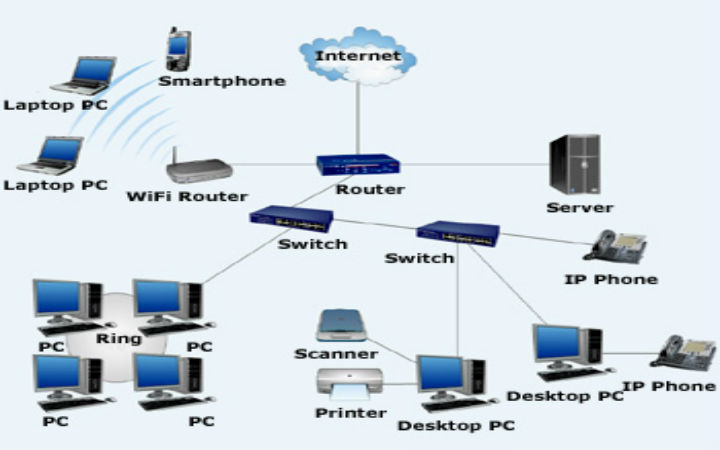
\includegraphics[scale=0.4,cframe=blue 0.5pt 3pt]{Working of Router.jpg}
                  \caption{Working of Routers}
            \end{figure}
            Routers are Network layers device having basic functionality of exchanging data packets among the networks.The network can be both  Local area or Wide area Network.The received IP packets are forwarded towards their destination using routing Tables , which is updated frequently through communication between routers. Other important roles of router are Load balancing, Firewall,packet filtering etc..
      }
\end{A}


%%%%%%%%%%%%%%%%%%%%%%%%%%%%%

%%%%%%%%%%%%%%%%%%%%%%22222222222222222222222222222
\begin{Q}
      {
            List out the basic configuration commands of router (that you have used in this lab) with their syntax and functions.\\
      }
\end{Q}
\begin{itemize}
      \item To move to Privileged EXEC mode from User EXEC mode \textbf{enable} is used  and to return back \textbf{disable} is used.
            \CMD{user interface modes.txt}{Router user interface modes}

      \item To configure Router Hostname  first we have to be at Privileged EXEC mode followed by \textbf{configure terminal} command and then following codes are executed and required hostname : AMRIT is set.
            \CMD{Hostname.txt}{Configuring Hostname}
      \item To configure ethernet interface, Privileged EXEC mode is used one of the important command is \textbf{ip address (ip) (subnet)}. All other codes and syntaxes are mentioned below:
            \CMD{Configure ethernet interface.txt}{Configuting Ethernet Interface}
\end{itemize}

%%%%%%%%%%%%%%%%%%%%%%%%%%%%%%%%%%%%%%%%%%%%%%%

%%%%%%%%%%%%%%%%%33333333333333333333333333333

\begin{Q}
      {
            Note down the observation of each steps with necessary commands specified in activity D
            mentioned above and comment on it.
      }
\end{Q}

\begin{itemize}
      \item \textbf{Activity D.1}

            First of all router is configured through terminal and all other PCs are configured with the help of IP configuration Option.For left  Switches GigabitEthernet 0/0 port is used and configured to \textbf{200.10.8.1} and for right GigabitEthernet 0/1 is used and configured to \textbf{200.10.9.1}. In all PCs the given ip are assigned with subnet mask \textbf{255.255.255.0} and default gateway \textbf{0.0.0.0}(default)

            \CMD{configure giga.txt}{Configuring Router for Left and right switches}

            And finally the following configuration is achieved.
            \begin{figure}[H]
                  \centering
                  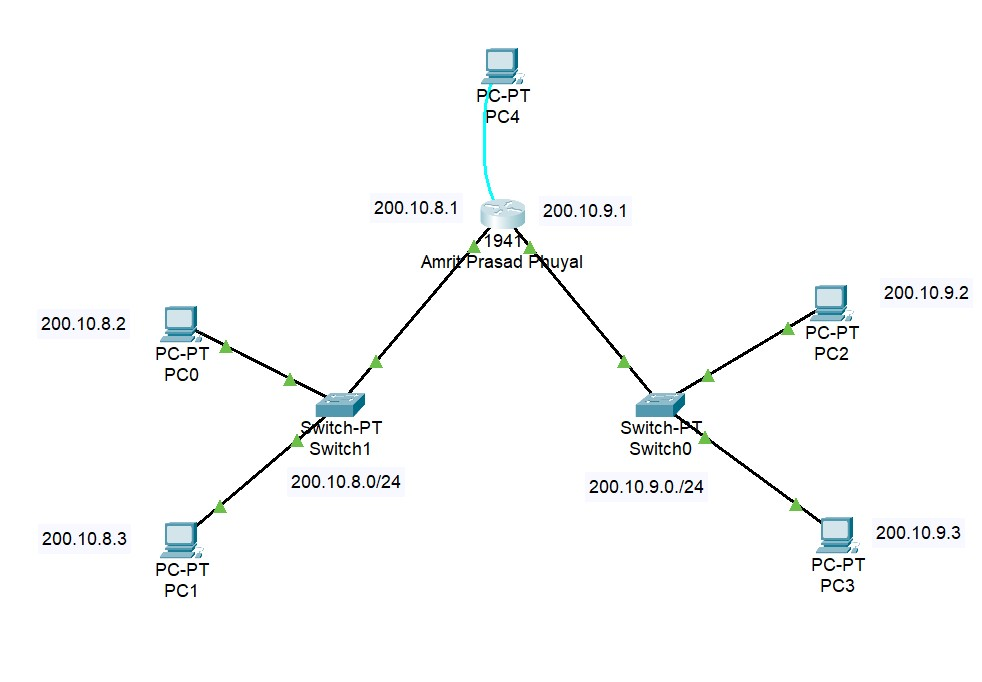
\includegraphics[scale=0.75,cframe=blue 0.5pt 3pt]{basic config.jpg}
                  \caption{Basic configuration and Setup}
            \end{figure}
            All PCs and Router IP's are listed below.

            \begin{table}[H]
                  \centering
                  \begin{tabular}{|c|c|}
                        \hline
                        \textbf{Name}      & \textbf{IP address} \\
                        \hline
                        GigabitEthernet0/0 & 200.10.8.1          \\
                        \hline
                        PC0                & 200.10.8.2          \\
                        \hline
                        PC1                & 200.10.8.3          \\
                        \hline
                        GigabitEthernet0/1 & 200.10.9.1          \\
                        \hline
                        PC2                & 200.10.9.2          \\
                        \hline
                        PC3                & 200.10.9.3          \\
                        \hline
                  \end{tabular}
            \end{table}
      \item \textbf{Activity D.2}

            Hostname is set to AMRIT as an identifier to the network.
            \CMD{Hostname.txt}{Changing Hostname to AMRIT}

      \item \textbf{Activity D.3}

            Performing Ping from PC0 to all other PCs and Router.
            \begin{itemize}
                  \item PCO to GigabitEthernet 0/0
                        \CMD{p0-r0.txt}{Ping PCO to GigabitEthernet 0/0}
                  \item PCO to PC1
                        \CMD{p0-1.txt}{Ping PCO to PC1}
                  \item PCO to GigabitEthernet 0/1
                        \CMD{p0-r1.txt}{Ping PCO to GigabitEthernet 0/1}
                  \item PCO to PC2
                        \CMD{p0-2.txt}{Ping PCO to PC2}
                  \item PCO to PC3
                        \CMD{p0-3.txt}{Ping PCO to PC3}
            \end{itemize}

      \item \textbf{Activity D.4}

            Performing Ping from PC3 to all other PCs and Router.
            \begin{itemize}
                  \item PC3 to GigabitEthernet 0/0
                        \CMD{p3-r0.txt}{Ping PC3 to GigabitEthernet 0/0}
                  \item PC3 to PC0
                        \CMD{p3-0.txt}{Ping PC3 to PC0}
                  \item PC3 to PC1
                        \CMD{p3-1.txt}{Ping PC3 to PC1}
                  \item PC3 to GigabitEthernet 0/1
                        \CMD{p3-r1.txt}{Ping PC3 to GigabitEthernet 0/1}
                  \item PC3 to PC2
                        \CMD{p3-2.txt}{Ping PC3 to PC2}
            \end{itemize}


      \item \textbf{Activity D.5}

            Performing Ping from Router to all other PCs.
            \begin{itemize}
                  \item Router to PC0
                        \CMD{pr-0.txt}{Router to PC0}
                  \item Router to PC1
                        \CMD{pr-1.txt}{Router to PC1}
                  \item Router to PC2
                        \CMD{pr-2.txt}{Router to PC2}
                  \item Router to PC3
                        \CMD{pr-3.txt}{Router to PC3}
            \end{itemize}

            %%%%%%%%%%%%%%%%%%%%%%%%%%%%%%%%%%%%%%%%%%%%%%%%%%%%%%%%%%%%%%%%%%%%%%%%%%%
            \HRule

            {\large Set the default gateway of PC0 and PC1 as \textbf{200.10.8.1} Similarly set the default gateway of PC2 and PC3 as \textbf{200.10.9.1 }and repeating activity D.3, D.4, D.5 once again }

            \HRule
            %%%%%%%%%%%%%%%%%%%%%%%%%%%%%%%%%%%%%%%%%%%%%%%%%%%%%%%%%%%%%%%%%%%%%%%%%%%%%
      \item \textbf{Repeating Activity D.3}

            Performing Ping from PC0 to all other PCs and Router.
            \begin{itemize}
                  \item PCO to GigabitEthernet 0/0
                        \CMD{gp0-r0.txt}{Ping PCO to GigabitEthernet 0/0}
                  \item PCO to PC1
                        \CMD{gp0-1.txt}{Ping PCO to PC1}
                  \item PCO to GigabitEthernet 0/1
                        \CMD{gp0-r1.txt}{Ping PCO to GigabitEthernet 0/1}
                  \item PCO to PC2
                        \CMD{gp0-2.txt}{Ping PCO to PC2}
                  \item PCO to PC3
                        \CMD{gp0-3.txt}{Ping PCO to PC3}
            \end{itemize}

      \item \textbf{Repeating Activity D.4}

            Performing Ping from PC3 to all other PCs and Router.
            \begin{itemize}
                  \item PC3 to GigabitEthernet 0/0
                        \CMD{gp3-r0.txt}{Ping PC3 to GigabitEthernet 0/0}
                  \item PC3 to PC0
                        \CMD{gp3-0.txt}{Ping PC3 to PC0}
                  \item PC3 to PC1
                        \CMD{gp3-1.txt}{Ping PC3 to PC1}
                  \item PC3 to GigabitEthernet 0/1
                        \CMD{gp3-r1.txt}{Ping PC3 to GigabitEthernet 0/1}
                  \item PC3 to PC2
                        \CMD{gp3-2.txt}{Ping PC3 to PC2}
            \end{itemize}


      \item \textbf{Repeating Activity D.5}

            Performing Ping from Router to all other PCs.
            \begin{itemize}
                  \item Router to PC0
                        \CMD{gpr-0.txt}{Router to PC0}
                  \item Router to PC1
                        \CMD{gpr-1.txt}{Router to PC1}
                  \item Router to PC2
                        \CMD{gpr-2.txt}{Router to PC2}
                  \item Router to PC3
                        \CMD{gpr-3.txt}{Router to PC3}
            \end{itemize}
\end{itemize}
%%%%%%%%%%%%%%%%%%%%%%%%%%%%%%%%%%%%%%%

Default gateway is the Hardware node that facilitate the connection betweens and among the networks. Previously  the default gateway for device connected to left switch was \textbf{0.0.0.0} though it is physically connected to GigabitEthernet 0/0 port of Router having assigned ip \textbf{200.10.8.1} and similarly for right side the default gateway was \textbf{0.0.0.0} though it is physically connected to GigabitEthernet 0/1 port of Router having assigned ip \textbf{200.10.9.1}\\

Due to this  problem PC0 can Ping PC1 But Unable to ping router or any devices on right sides (PC2,PC3), as without proper Default Gateway PC0 has  no idea how it can connect to a totally different network at right hand side .\\

BUT after changes to Default gateway was made  all PCs can Ping each other and  Router.


\section{Conclusion}
Lab exercises includes Basic Configuration, Changing Hostname ,Ping and Information about importance of Default gateway(Router) in Network . While pinging PC3 fom PC0 with Default Gateway \textbf{0.0.0.0} there was error as Packets cant reach the destination because the sender PC0 has wrong information about Path to be followed to reach PC3. Soon after the Default Gateway was corrected all PCs and Router can Ping Each other. The Packet tracer file is attached with this report.

\end{document}